% This text is proprietary.
% It's a part of presentation made by myself.
% It may not used commercial.
% The noncommercial use such as private and study is free
% Dec 2007
% Author: Sascha Frank 
% University Freiburg 
% www.informatik.uni-freiburg.de/~frank/
%
% 
\documentclass{beamer}
\setbeamertemplate{navigation symbols}{}
\usetheme{Warsaw}

\usepackage[export]{adjustbox}

\usepackage[thinlines]{easytable}

\beamersetuncovermixins{\opaqueness<1>{25}}{\opaqueness<2->{15}}

\def\mydot{\structure{\rule{1ex}{1ex}}\,}
\def\B#1{\mathbf{#1}}
\def\emph#1{\textbf{\textcolor{orange}{#1}}}
\def\photocredit#1{\vspace{-.5em}{\tiny \textit{(Picture is courtesy of #1)}}}
\def\leadto{$\mathbf{\implies}$}
\DeclareMathOperator{\argmin}{argmin}
\DeclareMathOperator{\prox}{prox}
\DeclareMathOperator{\proj}{proj}

\newcommand{\mycite}[1]{\textcolor{myblue}{\text{ [#1]}}}

%% put page number in slide footer
\newcommand*\oldmacro{}%
\let\oldmacro\insertshorttitle%
\renewcommand*\insertshorttitle{%
  \oldmacro\hfill%
  \insertframenumber\,/\,\inserttotalframenumber}

\definecolor{darkgreen}{rgb}{0,0.5,0}
\definecolor{myblue}{RGB}{102,153,255}
\definecolor{mygray}{RGB}{200,200,200}

\AtBeginSection[]{
  \begin{frame}
  \vfill
  \centering
  \begin{beamercolorbox}[sep=8pt,center,shadow=true,rounded=false]{title}
    \usebeamerfont{title}\insertsectionhead\par%
  \end{beamercolorbox}
  \vfill
  \end{frame}
}

\begin{document}

\setbeamertemplate{caption}{\raggedright\insertcaption\par}
\setlength\abovecaptionskip{-2pt}

\title{Modelling inter-subject functional variability}  
\author[\emph{Elvis Dohmatob}]{\emph{Elvis Dohmatob}\\
  (PhD supervised by B. Thirion and G. Varoquaux)}

% \logo{
%}

\institute{Parietal Team, INRIA}
\date{September 26, 2017} 


\begin{frame}
  \titlepage

  \begin{centering}
    
\includegraphics[width=.22\linewidth]{figures/unips_logo}\;
    
\includegraphics[width=.22\linewidth]{figures/inria_logo}\;
    
\includegraphics[width=.27\linewidth]{figures/parietal}\;
    
\includegraphics[width=.22\linewidth]{figures/neurospin_logo}\;
  \end{centering}
  
\end{frame}

  \setcounter{tocdepth}{1}

\begin{frame}\frametitle{Context}
  \mydot A major goal of human neuroscience is to understand
  \begin{itemize}
  \item the structure,
  \item function, and
  \item inter-subject variability of the human brain
  \end{itemize}

  \uncover<2->{
    \mydot We will focus on \textbf{\textcolor{blue}{inter-subject functional variability}}
  }
\end{frame}

  
\begin{frame}\frametitle{Table of contents}\tableofcontents
\end{frame} 

\section{Introduction} 
\subsection{Regions and functional networks}
\begin{frame}\frametitle{Brain function regions and networks}
  \begin{figure}
    \caption{\emph{Part of the language network}}
    
    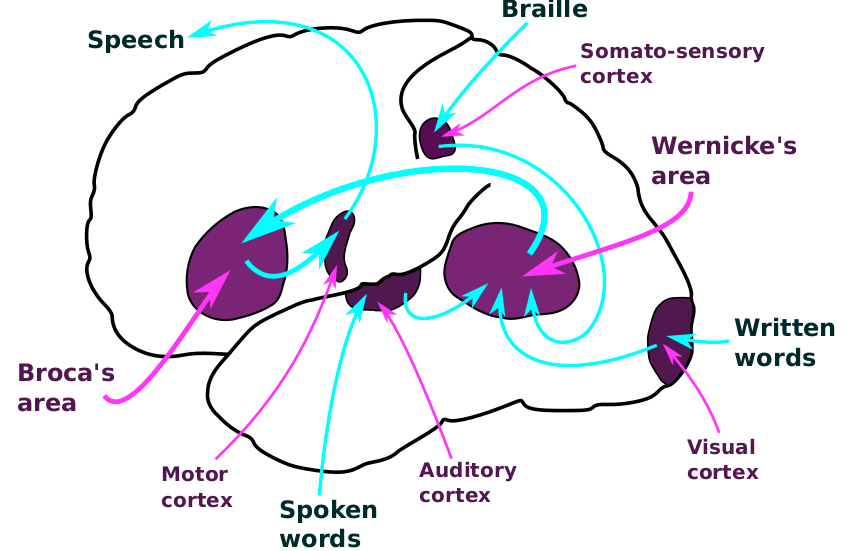
\includegraphics[scale=.3]{language}
  \end{figure}

\photocredit{Gael Varoquaux}
\end{frame}


\begin{frame}
  \frametitle{Mapping cognitive circuits in the brain}
  \begin{center}
  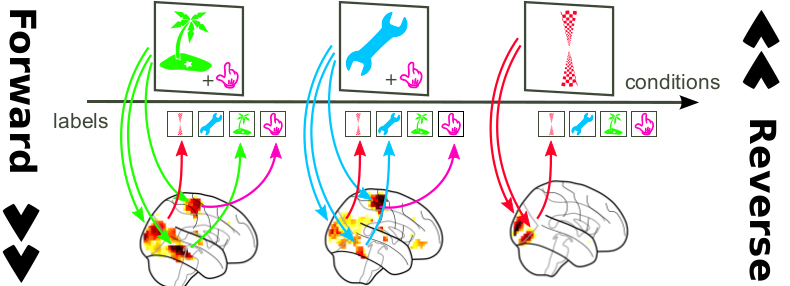
\includegraphics[width=.9\linewidth]{forwardback_inference.png}
\end{center}
\vspace{-1.em}
  \photocredit{Yannick Schwarz}

  \smallskip
  
  \mydot \emph{Forward inference} \mycite{Friston '95'} detects voxels responding to an experimental condition

  \uncover<2->{
    \mydot \emph{Reverse inference / brain-decoding} \mycite{Dehaene 98; Cox 03} predicts the experimental condition
    from brain signals
  }

  \uncover<3->{
    \mydot We will focus on \emph{reverse-inference / brain-decoding}
  }
    
\end{frame}



\subsection{Inter-subject functional variability}
\begin{frame}
  \frametitle{Variability in both location and magnitude of activations}
  \uncover<1->{\mydot
    % Group mean and individual activation maps,
    Story vs Math language contrast of HCP dataset \mycite{van Essen '12}}
  
  \medskip
  
\begin{overlayarea}{\textwidth}{\textheight}
  \only<1>{
    \centering
    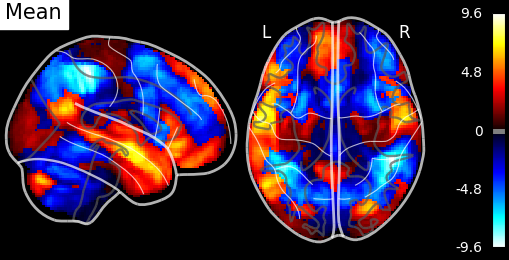
\includegraphics[width=0.34\linewidth]{intersubject_var_01.png}
  }
  \only<2>{
    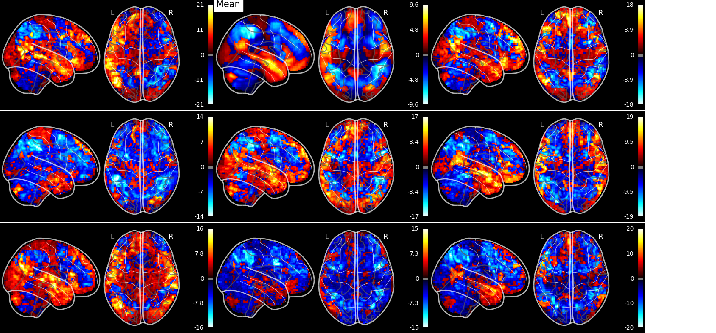
\includegraphics[width=1.1\linewidth]{intersubject_var_figure_00.pdf}
  }
\end{overlayarea}

  % 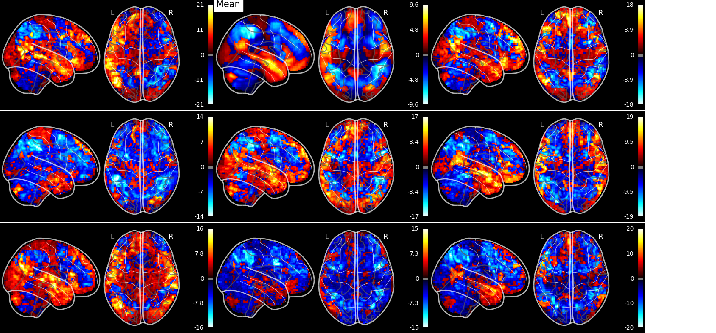
\includegraphics[width=1.1\linewidth]{intersubject_var_figure_00.pdf}
%   \begin{overlayarea}{\textwidth}{\textheight}
%     \only<1->{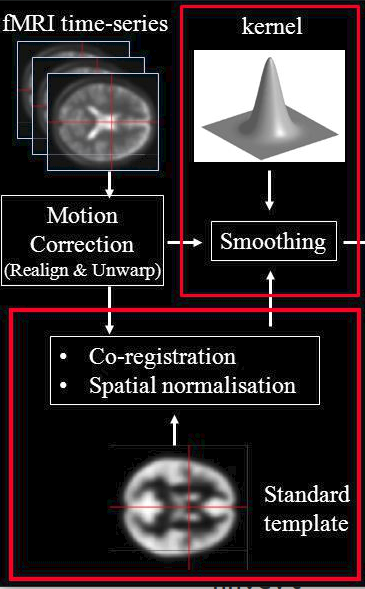
\includegraphics[width=.38\linewidth, valign=c]{preproc.png}\;}\only<2->{
\includegraphics[width=.2\linewidth, valign=c]{arrow.png}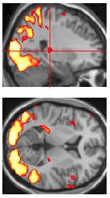
\includegraphics[width=.3\linewidth, valign=c]{statsmodel.png}}

%     \only<1->{\tiny \textit{(Adapted from Marion Oberhuber \& Giles Story)}
% }
%   \end{overlayarea}

\end{frame}

\begin{frame}
  \frametitle{Variability in both location and magnitude of activations}\Large
  \mydot Inter-subject functional variability \textcolor{red}{$\ne$} noise!
  \begin{itemize}
  \item Is predictive of behavioral differences between individuals
  \end{itemize}

  \bigskip
  
  \mydot Cannot be corrected via spatial normalization, etc.
\end{frame}

\subsection{Brain-decoding}
\begin{frame}\frametitle{A zoom on  brain-decoding}
  \begin{overlayarea}{\textwidth}{\textheight}
    \only<1->{
  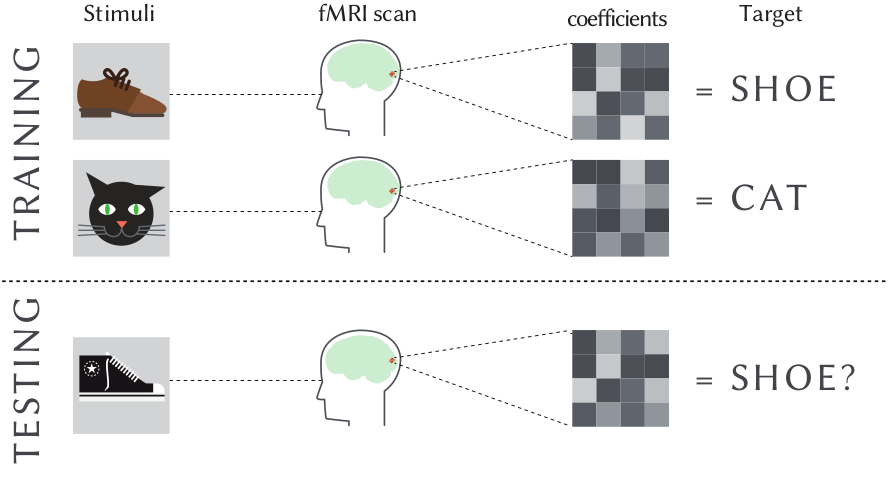
\includegraphics[width=.9\linewidth]{decoding.png}
        
  \quad\quad\quad$\B{y}_i$\quad\quad\quad\quad\quad\quad\;\;$\B{x}_i$
  \quad\quad\quad\quad\quad\quad\;$\B{w}$
  \quad\quad\quad\quad$\hat{\B{y}}_i$
}
    \medskip

\only<2->{    
    \mydot This is \emph{supervised machine-learning}
    
    \mydot We don't just want good predictions, we want \emph{regions}
  }
  \end{overlayarea}

% \mydot \emph{$\B{X}_i$}: each sample is a 3D MRI brain image scanned at a particular instant $i$.

% \mydot \emph{$\B{y}_i$}: target, the class of the stimulus at instant $i$.

% \mydot There are as many features as voxels (up to \textcolor{red}{$10^6$}).
\end{frame}


\section{Structured penalties for multi-variate brain-decoding}
\subsection{Preliminaries}

% \begin{frame}
%   \frametitle{Mapping cognitive circuits in the brain}
%   \begin{center}
%   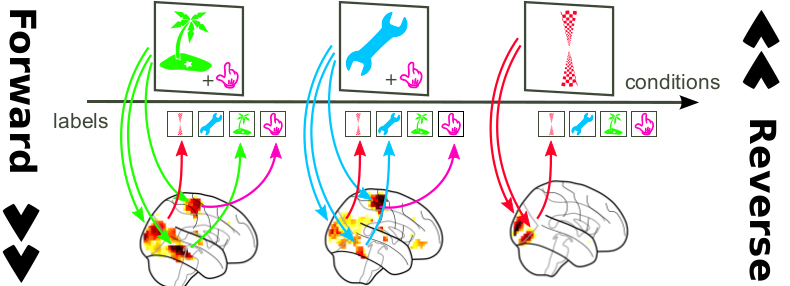
\includegraphics[width=.9\linewidth]{forwardback_inference.png}
% \end{center}
% \vspace{-1.em}
%   \photocredit{Yannick Schwarz}

%   \smallskip
  
%   \mydot \emph{Forward inference} \mycite{Friston '95'} detects voxels responding to an experimental condition

%   \uncover<2->{
%     \mydot \emph{Reverse inference / brain-decoding} \mycite{Dehaene 98; Cox 03} predicts the experimental condition
%     from brain signals
%   }

%   \uncover<3->{
%     \mydot We will focus on \emph{reverse-inference / brain-decoding}
%   }
  
  
% \end{frame}

% \begin{frame}\frametitle{A zoom on  brain-decoding}
%   \begin{overlayarea}{\textwidth}{\textheight}
%     \only<1->{
%   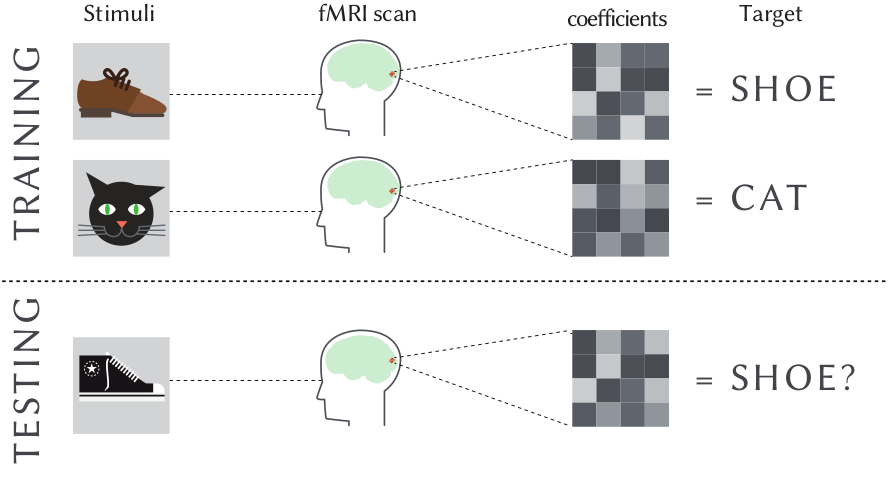
\includegraphics[width=.9\linewidth]{decoding.png}
        
%   \quad\quad\quad$\B{y}_i$\quad\quad\quad\quad\quad\quad\;\;$\B{x}_i$
%   \quad\quad\quad\quad\quad\quad\;$\B{w}$
%   \quad\quad\quad\quad$\hat{\B{y}}_i$
% }
%     \medskip

% \only<2->{    
%     \mydot This is \emph{supervised machine-learning}
    
%     \mydot We don't just want good predictions, we want \emph{regions}
%   }
%   \end{overlayarea}

% % \mydot \emph{$\B{X}_i$}: each sample is a 3D MRI brain image scanned at a particular instant $i$.

% % \mydot \emph{$\B{y}_i$}: target, the class of the stimulus at instant $i$.

% % \mydot There are as many features as voxels (up to \textcolor{red}{$10^6$}).
% \end{frame}

\begin{frame}\frametitle{What we mean by ``structured''}
  \begin{overlayarea}{\textwidth}{\textheight}
    \only<1->{
\begin{columns}
  \begin{column}{7.5cm}
    \emph{Definition:}
    
  \mydot Localized activation patterns -- \emph{sparsity}

  \medskip
  
  \mydot Clusters of active voxels -- \emph{smoothness}
\end{column}
\begin{column}{5cm}
    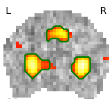
\includegraphics[width=.6\linewidth]{structure.png}
\end{column}
\end{columns}
}

\medskip
\hrule
\medskip
\only<2->{
  
  \hspace{-2.3em}\mydot Such a model is much more \emph{interpretable} (i.e small number of \emph{regions}) than classical methods like SVM, Ridge regression, Lasso

  \medskip
  
  \hspace{-2.3em}\mydot Performs \emph{model-estimation} and \emph{feature-selection} jointly

  \medskip

  \hspace{-2.3em}\mydot Fights the \emph{curse-of-dimensionality}, via dimensionality reduction.
  }
\end{overlayarea}
\end{frame}

\subsection{Spatial priors for brain decoding}
\begin{frame}\frametitle{Generalized linear models with structured penalties}
  \vspace{-1.3em}
  \begin{overlayarea}{\textwidth}{\textheight}
    \only<1->{    
  \begin{columns}
    \column{.68\linewidth}
  {\centering
    \huge
    $ \underset{\mathbb E [\B{y}|\B{x}_i]}
    {
\includegraphics[width=.2\linewidth, valign=c]{cat.png}} = f\left(
      \underset{\B{w}}{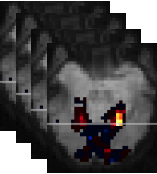
\includegraphics[width=.2\linewidth, valign=c]{w.png}}\;\underset{\B{x}_i}{
\includegraphics[width=.2\linewidth, valign=c]{3Dfmri.png}}\right)      
    $
}
% \hspace{-2em}
\column{.47\linewidth}
\uncover<2->{
  
    \mydot \emph{Samples} $\B{x}_1,\ldots,\B{x}_n \in \mathbb R^p$
    \begin{itemize}
    \item \# samples $n \sim \textcolor{red}{10^3}$
    \item \# \emph{features} $p \sim \textcolor{red}{10^6}$ voxels
    \end{itemize}
  }
  \uncover<3->{
    \mydot Model \emph{weights} $\B{w} \in \mathbb R^p$
  }

\uncover<4->{
  
    \mydot $f = \text{"logit"}$ in \emph{classification}
    
    \mydot $f = \text{"id"}$ in \emph{regression}
  }  
  \end{columns}
}
\medskip

  \uncover<4->{
    \mydot Optimization problem:
    \vspace{-.8em}
    \[
      \min_{\B{w} \in \mathbb R^p}%\left\{E(\B{w}) :=
      \underbrace{\frac{1}{n}\sum_{i=1}^n \ell({y}_i, f(\langle \B{w}, \B{x}_i\rangle))}_{\text{\emph{data / loss term}}} + \underbrace{\alpha\mathcal P(\B{w})}_{\text{penalty}}%\right\}
    \]
  }
  \uncover<5->{

  \vspace{-1em}  
    \mydot \emph{$\ell({y}_i,f(\B{x}_i^T\B{w}))$} $=
    \begin{cases}\frac{1}{2}(y_i-\langle \B{w}, \B{x}_i\rangle)^2, &\mbox{ \text{ in regression}},\\
      \log(1+\exp(-{y}_i\langle \B{w}, \B{x}_i\rangle)), &\mbox{ \text{ in classif. (OvR)}}\\
      % &\mbox{ \text{ {(log. reg.)}}}\\
      % (1-y_i\B{x}_i^T\B{w})_+,&\mbox{ \text{(hinge)}}\\
      % \vdots\\
    \end{cases}
    $
  }
\end{overlayarea}
% \mydot \textcolor{green}{{$\ell(\B{y}, \B{X} \B{w})$}} is the
% \emph{loss} term
%   $$
%   \ell(\B{y},\B{X}\B{w}) =
%   \frac{1}{n}\sum_{i=1}^n 
%   \begin{cases}\frac{1}{2}(\B{x}^T_i\B{w} - y_i)^2
%     %= \frac{1}{2}(\B{X}^T_i\B{w} - \B{y}_i)^2
%     ,
%     &\mbox{ \text{ (least sq.)}}\\
%     \log(1+\exp(-{y}_i\B{x}_i^T\B{w})),
%     &\mbox{ \text{ {(log. reg.)}}}\\
%     % (1-y_i\B{x}_i^T\B{w})_+,&\mbox{ \text{(hinge)}}\\
%     \vdots\end{cases}
%   $$
\end{frame} %--------------------------------------------------------------}}}

\begin{frame}\frametitle{Spatial penalties impose structure in the model}
\vspace{-1.2em}  
  \begin{overlayarea}{\textwidth}{\textheight}  
    \uncover<1->{
      $\underset{\B{w} \in \mathbb R^p}{\text{min }}%\left\{E(\B{w}) :=
      \underbrace{\frac{1}{n}\sum_{i=1}^n \ell(\B{y}_i, f(\langle \B{w}, \B{x}_i\rangle))}_{\text{data / loss term}} + \underbrace{\alpha\mathcal P(\B{w})}_{\emph{\text{penalty}}}%\right\}
      \;\;\vline\;\;
    }
    \uncover<3->{
      \underset{\text{structured penalty}}{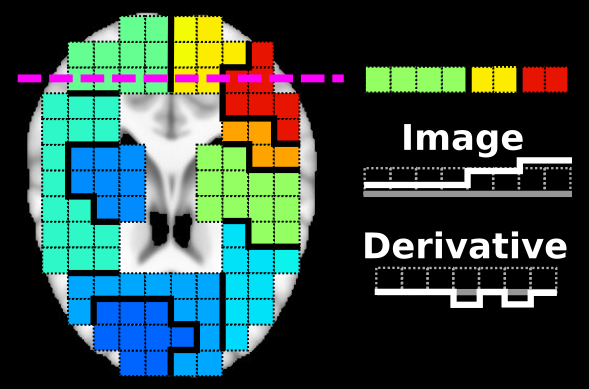
\includegraphics[width=.23\linewidth, valign=c]{cartoon}}\;
\includegraphics[width=.05\linewidth, valign=c]{arrow}\;
      \underset{\quad\;\;\;\B{w}}{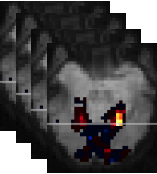
\includegraphics[width=.17\linewidth, valign=c]{w.png}}
    }$

    \uncover<3->{
      \vspace{-.5em}
      \[
%      \begin{split}
        \hspace{-1em}\mathcal P(\B{w}) = \begin{cases}
          % \rho\|\B{w}\|_1 + \frac{1}{2}(1-\rho)\|\nabla \B{w}\|_{\text{Fro}}^2 =
          \sum_{j \in [\![p]\!]}\rho|\B{w}_j| + \frac{1}{2}(1-\rho)\|(\nabla \B{w})_j\|_2^2, &\mbox{ \emph{GraphNet},
            % ~\citep{grosenick2013,hebiri2011}
          }\\
    % \|\nabla_\rho \B{w}\|_{1+2,1} =
    % \rho\|\B{w}\|_1 + \|\nabla \B{w}\|_{2,1} =
    \sum_{j  \in [\![p]\!]}\rho|\B{w}_j| + (1-\rho)\|(\nabla \B{w})_j\|_2, &\mbox{ \emph{isotropic TV-L1},
    % ~\citep{baldassarre2012,gramfort2013}
    }\\
    % \|\nabla_\rho \B{w}\|_{1,1} =
    % \rho\|\B{w}\|_1 + (1-\rho)\|\nabla \B{w}\|_{1,1} =
    % \sum_{j  \in [\![p]\!]}\rho|\B{w}_j| + (1-\rho)\|(\nabla \B{w})_j\|_1, &\mbox{ anisotropic TV-$\ell_1$
  % }\\
  %   \|\nabla_\rho \B{w}\|_{2,1} =
    \sum_{j \in [\![p]\!]}(\rho^2|\B{w}_j|^2 + (1-\rho)^2\|(\nabla \B{w})_j\|_2^2)^{1/2},
    % \sum_{j  \in [\![p]\!]}\|(\nabla_\rho \B{w})_j\|_2,
    &\mbox{ \emph{Sparse Variation},
      %~\citep{eickenberg2015total}
    }
    \\\vdots
    \end{cases}
 % \end{split}
\]    
}

\vspace{-1em}
\uncover<4->{
  \mydot {Bayesian interpretation}
  \vspace{-.5em}
 \begin{eqnarray*}
   \begin{split}
     \underbrace{P(\B{w} | \B{x}_i,y_i)}_{\text{\emph{posterior}}} &\propto \underbrace{P(y_i|\B{x}_i,\B{w})}_{\text{\emph{likelihood}}}\underbrace{P(\B{w})}_{\text{\emph{prior}}}
     \propto \exp(-\ell(y_i,f(\langle \B{w},\B{x}_i\rangle)))\exp(-\alpha\mathcal P(\B{w}))
   \end{split}
 \end{eqnarray*}
}
\end{overlayarea}
\end{frame}

\begin{frame}\frametitle{References for the penalties}\Large
  \bigskip
 \mydot Total-Variation (TV) \mycite{Michel '11}

   \bigskip

   \mydot TV-L1 \textcolor{myblue}{[Baldassare '12, Gramfort '13]}

  \bigskip
   
 \mydot GraphNet / S-Lasso \mycite{Hebiri '11, Grosenick
     '13}

   
  \bigskip
   
 \mydot Sparse-Variation \textcolor{myblue}{[Eickenberg '15]}
 
\end{frame}

\begin{frame}
  \frametitle{Spatial penalties \leadto more interpretable brain maps}
  % Faces vs objects classification on \textcolor{myblue}{[Haxby 2001]}
  \centering
  {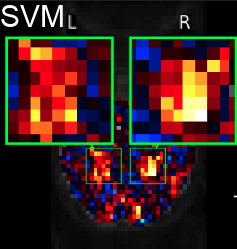
\includegraphics[width=.28\textwidth]{svm_with_title.png}}

  \medskip
  
  \hrule
  
  \medskip
  {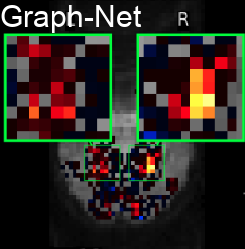
\includegraphics[width=.28\textwidth]{graphnet_with_title.png}}
  {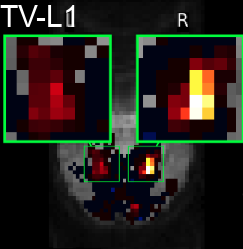
\includegraphics[width=.28\textwidth]{tvl1_with_title.png}}

\end{frame}

\subsection{Algorithms}
\begin{frame}
  \frametitle{Penalties \leadto interpretable maps only if well-optimized}
  \uncover<1->{
    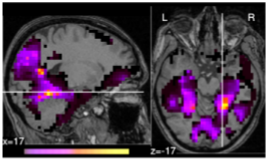
\includegraphics[width=.31\linewidth]{01.png}%
    \llap{\color{white}\raisebox{.15\linewidth}{\rlap{\sffamily
          $\Delta E < 10^{-1}$}}\hspace*{.31\linewidth}}\hfill%
  }
  \uncover<3->{
    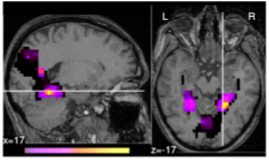
\includegraphics[width=.31\linewidth]{001.png}%
    \llap{\color{white}\raisebox{.15\linewidth}{\rlap{\sffamily
          $\Delta E < 10^{-3}$}}\hspace*{.31\linewidth}}\hfill%
  }
  \uncover<4->{
    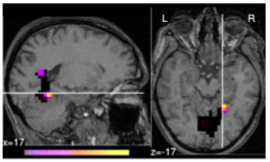
\includegraphics[width=.31\linewidth]{00001.png}%
    \llap{\color{white}\raisebox{.15\linewidth}{\rlap{\sffamily
          $\Delta E < 10^{-5}$}}\hspace*{.31\linewidth}}%
    }

\bigskip

\uncover<4->{
  \mydot Structured penalties $\implies$ \emph{more interpretable models}
}

\bigskip

\uncover<5->{
  \mydot Corresponding optim. problem is much \emph{harder} (than SVM, etc.)
  \begin{itemize}
    \item \emph{high-dimensional non-smooth ill-conditioned} problem
    \item Can't compute \emph{prox operator} analytically
  \end{itemize}
}

\bigskip

\uncover<6->{
\mydot Lack of fast solver can lead to \emph{wrong conclusions about model}
}

\bigskip

\uncover<7->{
  \mydot We need \emph{fast solvers!}
}
\end{frame}

\begin{frame}
  \frametitle{Our contributions}\Large
  \bigskip
  \bigskip
  \bigskip
  \centering
  \begin{beamerboxesrounded}{\emph{Faster, better, stronger!}}
    We propose a combination of \emph{algorithmic} and \emph{implementation} improvements that make these models usable out-of-the-box
  \end{beamerboxesrounded}
  
\end{frame}

\begin{frame}
  \frametitle{Looking for the ideal solver}
  % \vspace{-.5em}
  \mycite{Dohmatob '14, '15 (PRNI); Varoquaux '15 (Gretsi)}
  \medskip

  \mydot Solver speed sensitive to hyper-parameter

  \medskip      
\mydot Retained strategy is nested \textcolor{red}{FISTA} \mycite{Beck '09} algorithm
  
  % \vspace{-.5em}

  % \begin{overlayarea}{\textwidth}{\textheight}
  %   \only<1>{
  %     \begin{figure}
  %       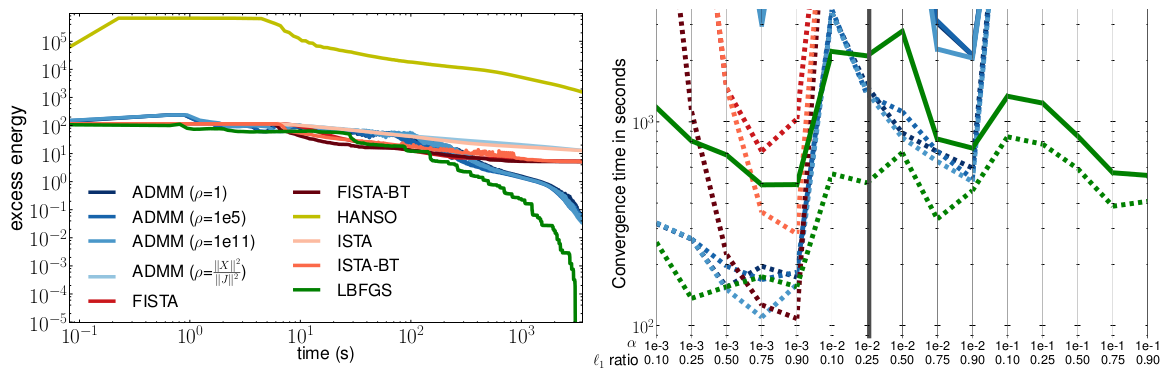
\includegraphics[width=1.05\linewidth]{figures/solvers_1.png}
  %       \caption{Classification: Visual recognition task \mycite{Haxby '01}
  %       }
  %     \end{figure}
  %   }
  %   \only<2->{
      \begin{figure}
        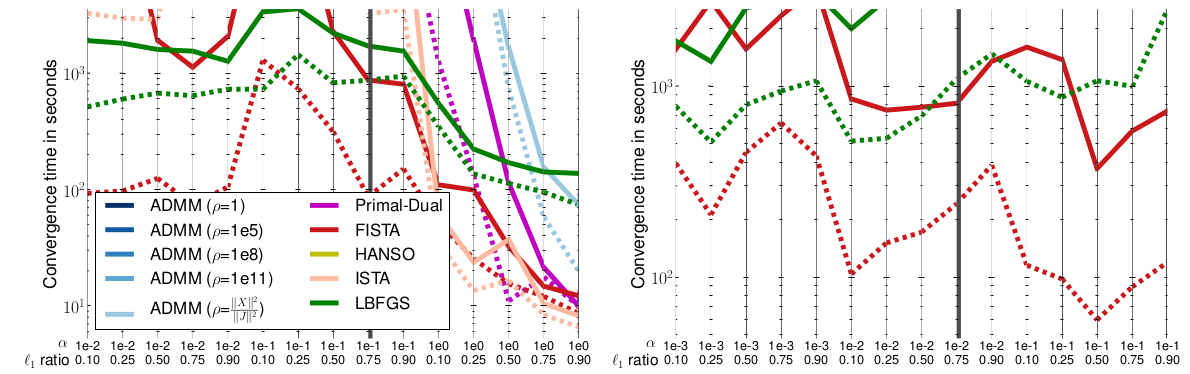
\includegraphics[width=1.05\linewidth]{figures/solvers_2.png}
        \caption{Benchmarks on ``mixed-gambles'' task \mycite{Jimura '12}}
      \end{figure}
    % }

    % \bigskip
    % \only<3->{
      % }
      
    % \end{overlayarea}
  
\end{frame}

\begin{frame}\frametitle{More speed via univariate feature-screening}
  \vspace{-.7em}
  \mycite{Dohmatob '15 (PRNI)}
  \medskip
  
  \mydot \emph{$t_k$} := $k$th percentile of the vector $|\B{X}^T\B{y}| := (|\B{x}_1^T\B{y}|,\ldots,|\B{x}_p^T\B{y}|)$.
  
  \mydot Discard $j$th voxel if \emph{$|\B{x}^T_j\B{y}| < t_k$}
  \bigskip
  
  \quad\textcolor{blue}{$k = 10\%$}\quad\quad\quad\;\textcolor{blue}{$k = 20\%$}\quad\quad\quad\textcolor{blue}{$k = 50\%$}\quad\quad\quad\textcolor{blue}{$k = 100\%$}
  \begin{overlayarea}{\textwidth}{\textheight}
    \only<1>{
    \begin{figure}
      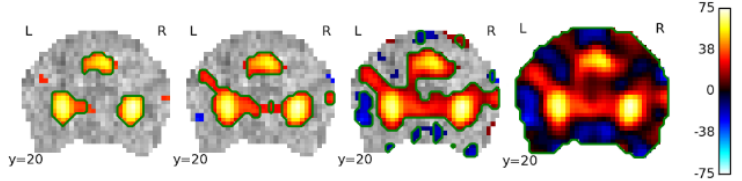
\includegraphics[width=\linewidth]{screening_gambling.png}
      \caption{Mixed gambling}
    \end{figure}
  }
  \only<2>{
    \vspace{-1em}
    \begin{figure}
      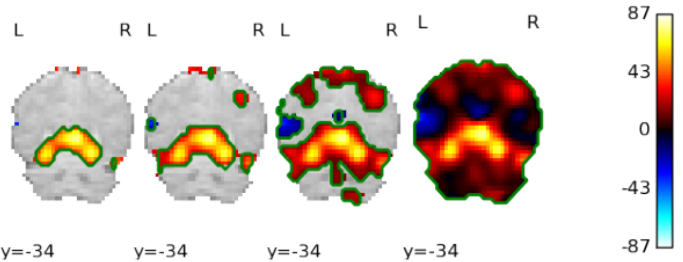
\includegraphics[width=\linewidth]{screening_haxby.png}
      \caption{Visual recognition}
    \end{figure}
  }

  \only<3>{
    \begin{figure}
      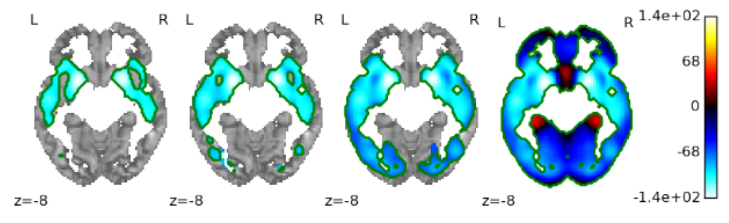
\includegraphics[width=\linewidth]{screening_oasis.png}
      \caption{Age prediction from gray-matter maps}
    \end{figure}
  }
  \end{overlayarea}

% \mydot Marginal screening \textcolor{myblue}{[Lee 2014]}, but \textcolor{red}{without} the
% (invertibility) restriction \emph{$k \le min(n, p)$}.

\end{frame}

\begin{frame}\frametitle{More speed via univariate feature-screening: results}
  \begin{columns}
    \column{.6\linewidth}
    \begin{overlayarea}{\textwidth}{\textheight}
      \only<1>{
          \mydot Age prediction
        
        \begin{figure}
          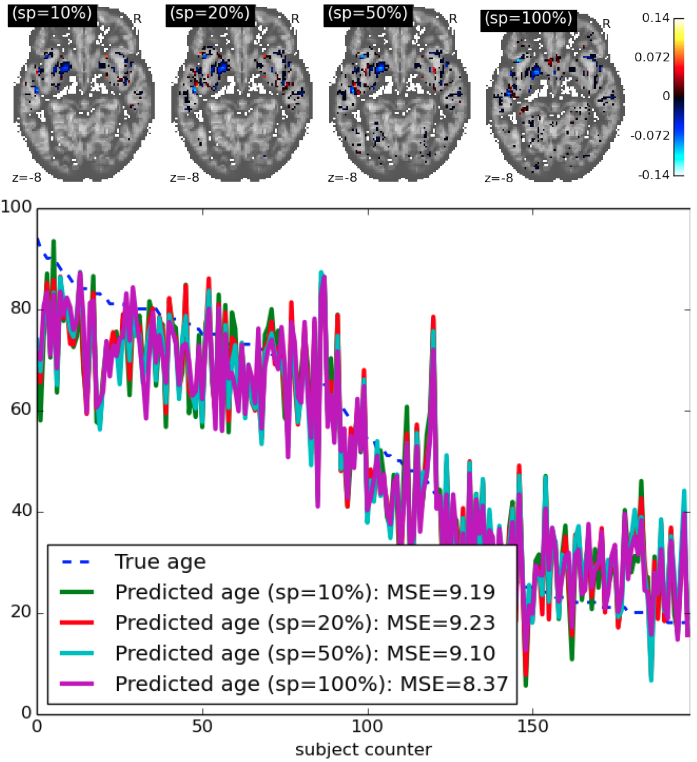
\includegraphics[width=1\linewidth]{figures/screening_oasis.png}
        \end{figure}
        \begin{table}[H]
          \begin{tabular}{|c|c|c|c|c|}\hline%\hline
            {$p$} & 100\% & 50\% & 20\% & 10\% \\ \hline
            {MSE} & 8.37 & 9.10 & 9.23 & 9.19 \\ \hline
          \end{tabular}
          \vspace{.3em}
        \end{table}
          
      }
      \only<2->{
        \mydot Visual object recognition % \mycite{Haxby 2001}
        
        \begin{figure}
          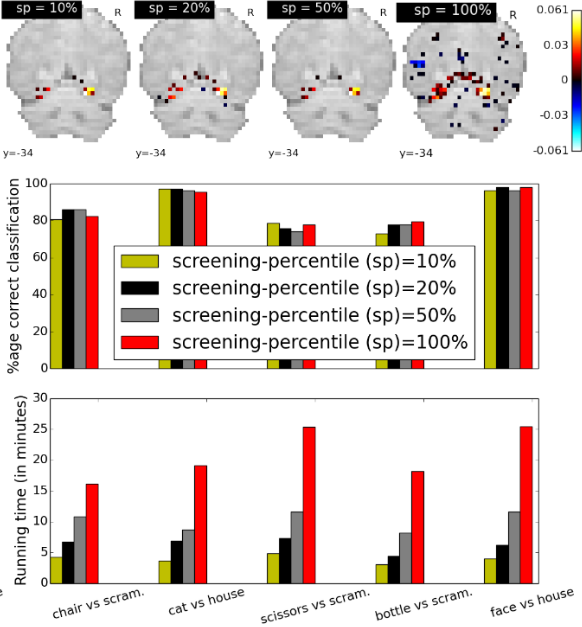
\includegraphics[width=.8\linewidth]{figures/haxby_sp.png}
        \end{figure}        
      }      
    \end{overlayarea}
    \column{.5\linewidth}
    \mycite{Dohmatob '15 (PRNI)}
    \bigskip
    
    % \mydot True model support approximated by screening procedure

    \mydot Solve on subset of features
    
    \bigskip
    
    \mydot Reduced training time

    \bigskip
    
    \mydot ...
  \end{columns}
 
\end{frame}


\begin{frame}\frametitle{Early-stopping}
  \begin{columns}    
    \column{.7\linewidth}
\mydot Stop optimization if accuracy on validation data stops improving \mycite{Dohmatob '15 (PRNI)}
    
    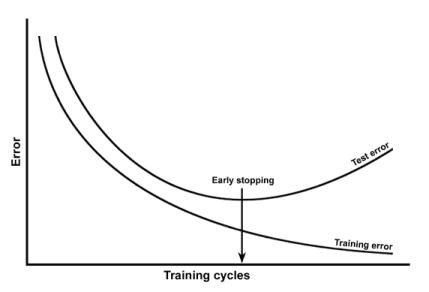
\includegraphics[width=1\linewidth]{early-stopping-graphic}
    \column{.45\linewidth}
    \mydot old idea (e.g \mycite{Bottou})

    \bigskip
    
    \mydot saves training time
    \bigskip
    
    \mydot implicit regularization

    \bigskip

    \mydot helps against overfitting

    \bigskip

    \uncover<2->{
      \mydot it's a % computational
    compromise
    \begin{itemize}
    \item it doesn't destroy accuracy
    \item but may lead to sub-optimal brain maps
    \end{itemize}
  }
  \end{columns}
\end{frame}

\begin{frame}\frametitle{Early-stopping: results}
  \vspace{-1.1em}
  \begin{columns}
    \column{.55\linewidth}
    \begin{overlayarea}{\textwidth}{\textheight}
      \only<1>{
        \begin{figure}
          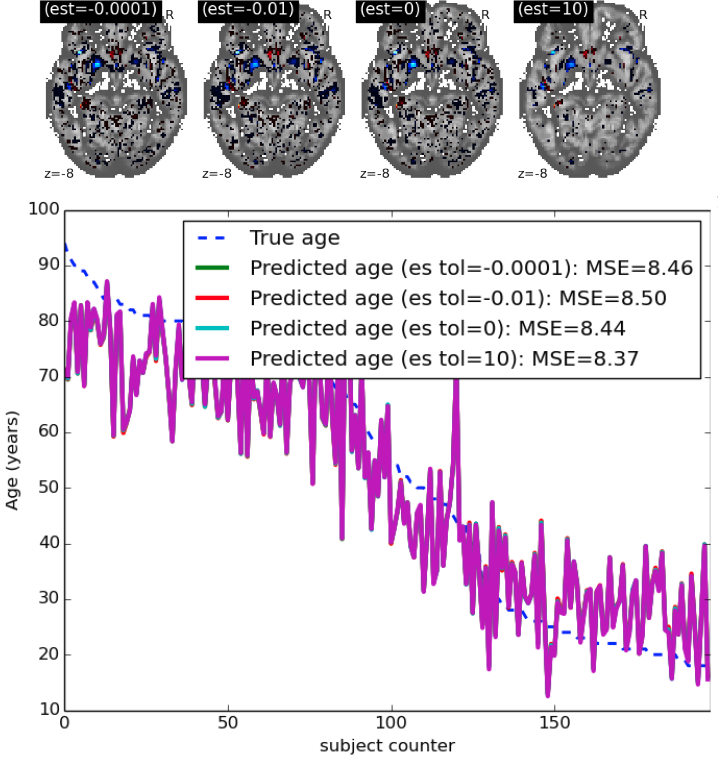
\includegraphics[width=1\linewidth]{figures/es_oasis.png}
        \end{figure}
      }
      \only<2->{
        \mydot Visual object recognition % \mycite{Haxby 2001}
        \begin{figure}
          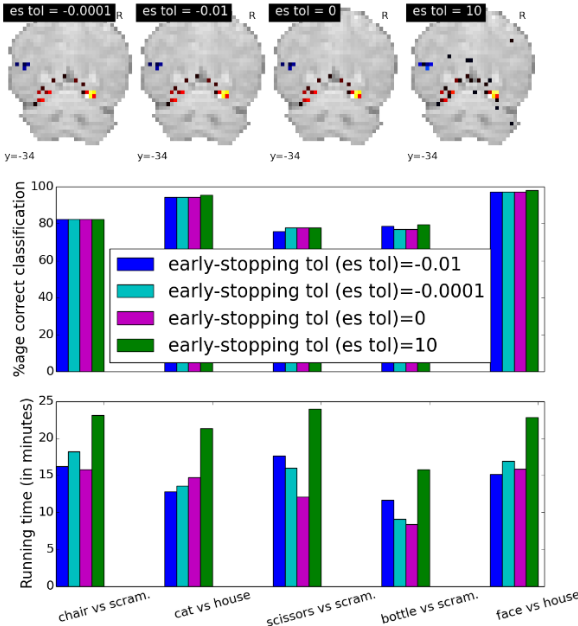
\includegraphics[width=.9\linewidth]{figures/haxby_es.png}
        \end{figure}
      }      
    \end{overlayarea}
    \column{.45\linewidth}
    \mycite{Dohmatob '15 (PRNI)}
    \bigskip
    
    % \mydot True model support approximated by screening procedure

        \mydot Solve on subset of features

        \bigskip 
    \mydot Yields up to \emph{x10 speedup!}

    \bigskip
    
    \mydot No significant loss in accuracy
  \end{columns}
 
\end{frame}

% \begin{frame}
% \frametitle{Results}
% \vspace{-.5em}
% \centering
%     {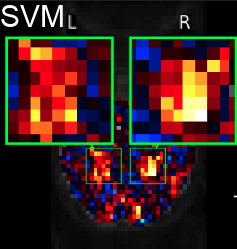
\includegraphics[width=.28\textwidth]{svm_with_title.png}}

%     \medskip

%     \hrule

%     \medskip
%     {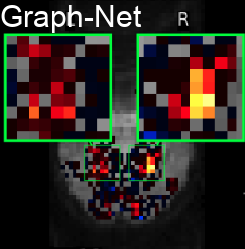
\includegraphics[width=.28\textwidth]{graphnet_with_title.png}}
%     {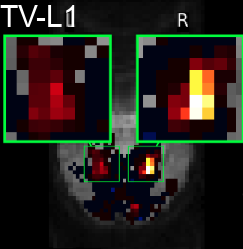
\includegraphics[width=.28\textwidth]{tvl1_with_title.png}}
% \end{frame}

\begin{frame}\frametitle{Section wrap-up}
  \mydot Building on prior work, we have developed enhanced structured penalties for multi-variate brain-decoding

  \bigskip
  
  \mydot Such penalties lead to more interpretable brain maps (localized blobs)

  \bigskip
  
  \mydot Focus on practical usability (fast model training)

  \bigskip
  
  \mydot Our contributions are available as part of \emph{Nilearn} toolkit.
  
\end{frame}

\section{Modelling inter-subject variability via dictionary-learning}
\subsection{Preliminaries}
\begin{frame}
  \frametitle{Learn latent model for inter-subject variability}
  % \vspace{-2em}
  \mydot \emph{Goal:} Learn a latent model of inter-subject functional variability
    \begin{equation*}
      \begin{split}
        % \B{X} &= \B{D} \times \B{C}\\
        \underset{\text{individual maps }(\B{X})}{\includegraphics[width=.26\linewidth, valign=c]{acti.pdf}} &=  \underset{\text{loadings }(\B{C})}{
\includegraphics[width=.235\linewidth, valign=c]{codes.pdf}} \times \;\underset{\text{dictionary }(\B{D})}{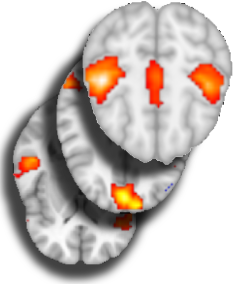
\includegraphics[width=.22\linewidth, valign=c]{dico.pdf}}
      \end{split}
    \end{equation*}
    \mydot Each \emph{cognitive map} $\B{x}_i$ with $p$ voxels gets \emph{encoded} over a \emph{dictionary} $\B{D}$ as $k$ \emph{loading coefficients} $\B{c}_i$,
    with $k \ll p$
\end{frame}  


\begin{frame}
  \frametitle{The challenge}\Large
\mycite{Dohmatob '16 (NIPS)}

  \bigskip

  \uncover<2->{
  \mydot \textcolor{red}{Sparsity:} spatially localized atoms
}
  \bigskip

  \uncover<3->{
  \mydot \textcolor{red}{Spatial blobs:} each atom = interpretable blobs
}

  \bigskip

  \uncover<4->{
    \mydot \textcolor{red}{Scalable / online:} model should trainable online
    }
\end{frame}


\subsection{Introducing the proposed model}
\begin{frame}
  \frametitle{Introducing the proposed model \textcolor{orange}{[Dohmatob '16 (NIPS)]}}
  \vspace{-2.1em}
  \begin{equation*}
    \begin{split}
      \underset{\B{X}}{\includegraphics[width=.26\linewidth, valign=c]{acti.pdf}} &=  \underset{\B{C}}{
\includegraphics[width=.235\linewidth, valign=c]{codes.pdf}} \times \;\underset{\B{D}}{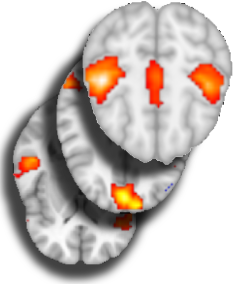
\includegraphics[width=.22\linewidth, valign=c]{dico.pdf}}
      \end{split}
  \end{equation*}
\vspace{-1em}
\begin{eqnarray*}
  \begin{split}
    &\min_{\B{D} \in \mathbb R^{p \times k}}\left(\lim_{n \rightarrow \infty}\frac{1}{n}\sum_{t=1}^n\min_{\B{c}_t \in \mathbb R^{k}}\frac{1}{2} \|\B{x}_t-\B{D}\B{c}_t\|_2^2 +  \frac{1}{2}\alpha\|\B{c}_t\|_2^2\right) \uncover<3->{+ \textcolor{orange}{\gamma\sum_{j=1}^k\Omega_{\text{Lap}}(\B{d}^j)}}\\
    &\uncover<2->{\textcolor{orange}{\text{subject to } \B{d}^1,\ldots,\B{d}^k \in \mathcal K}\mycite{Mairal '09'}}\uncover<3->{\quad\quad\quad\quad\quad\quad\quad\mycite{Dohmatob '16'}}
  \end{split}
\end{eqnarray*}

% \emph{\textbf{N.B.:}} You may see this a s kind of online PCA with structural constraints on the components / atoms.

\uncover<2-> {
  \mydot $\mathcal K \subseteq \mathbb R^p$ is an $\ell_1$ ball

  \mydot $\Omega_{\text{Lap}}(\B{d}^j) := \frac{1}{2}\|\nabla \B{d}^j\|_F^2$, penalty that \emph{imposes blobs} in atoms $\B{d}^j$.
}

\end{frame}


\subsection{Algorithms}
\begin{frame}\frametitle{Reminder on coordinate-descent (CD)}
  % \vspace{-1em}
  \mydot Optimize w.r.t  a variable, and then w.r.t to another, and so on ...
  \centering
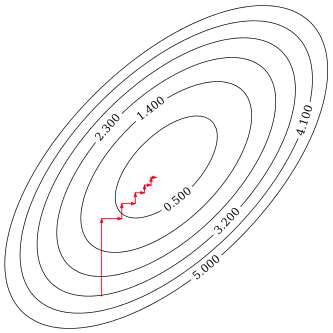
\includegraphics[width=0.5\linewidth]{cd.png}
  

\end{frame}

\begin{frame}
  \frametitle{The proposed algorithm}
  \rlap{\smash{
\includegraphics[width=1.5em]{loop}}}%
  \vspace{-1em}
  \begin{itemize}
\uncover<2->{    
\item \emph{Draw a sample} 3D brain image (or mini-batch) $\B{x}_t \in \mathbb R^p$
}
\uncover<3->{
\item \emph{Compute loadings} (i.e representation w.r.t current dict. $\B{D}$)
  \[
    \B{c}_t \leftarrow \argmin_{\B{u} \in \mathbb R^k}\frac{1}{2}\|\B{x}_t -
    \B{D} \B{u}\|_2^2 + \frac{1}{2}\alpha\|\B{u}\|_2^2.
  \]
}
\uncover<4->{
  \vspace{-1em}
    \item \emph{Rank-1 }updates: $\B{A}_t = \B{A}_{t-1} + \B{c}_t\B{c}_t^T$, $\B{B}_t := \B{B}_{t-1} + \B{x}_t\B{c}_t^T$
}
\uncover<5->{
  \item \emph{BCD dictionary update }of dictionary atoms

    \mydot \emph{Precompute} $\B{R} \leftarrow \B{B} - \B{D}\B{A}$

    \mydot
    \vspace*{.5em}
    \hspace{.1em}\rlap{\smash{
\includegraphics[width=1em]{loop}}}%
    \quad\emph{ for} $j = 1,2,\ldots,k$
  }
  \uncover<6->{
    
    % \quad\quad\quad\emph{\# Update} $j$th atom of dictionary % (few FISTA iters.)

    \quad\quad\quad\mydot \emph{Rank-1 }update: $\B{R} \leftarrow \B{R} + \B{d}^j \circ \B{a}^j$
    
    \quad\quad\quad\mydot \emph{FISTA loop: } $\B{d}^j \leftarrow
    \argmin_{\B{d} \in \mathcal K}F_{\gamma_t}(\B{d}, a_{j,j}^{-1}\B{r}^j)
    % = \prox_{(\textcolor{red}{F_{\gamma_t} + i_{\mathcal K}})}(a_{j,j}^{-1}\B{r}^j)
    $

    \quad\quad\quad\mydot \emph{Rank-1 }update: $\B{R} \leftarrow \B{R} - \B{d}^j \circ \B{a}^j$
  }    
\end{itemize}
  \hrule
  \bigskip

  \uncover<7->{
  \mydot \emph{N.B.:} $F_{\gamma_t}(\B{d},\B{z}) := \frac{1}{2}\|\B{d} - \B{z}\|_2^2
  + \frac{1}{2}\gamma_t\|\nabla\B{d}\|_{\text{F}}^2$, $\gamma_t := \gamma (a_{j,j}/t)^{-1}$

  }
  
\end{frame}

\subsection{Results}
\begin{frame}
  \frametitle{Experimental results on HCP fMRI data: qualitative}
  \begin{overlayarea}{\textwidth}{\textheight}
  \only<1->{
    \includegraphics[width=0.32\linewidth]{{figures/components_LANGUAGE_nc=40_PCA_7}.png}
  }
  \only<2->{
    \includegraphics[width=0.32\linewidth]{{figures/components_LANGUAGE_nc=40_alpha=auto_gamma=0_radius=4_split=0_time=12_29}.png}
  }
  \only<3->{
  \includegraphics[width=0.32\linewidth]{{figures/components_LANGUAGE_nc=40_alpha=auto_gamma=1000_radius=4_split=0_time=12_29}.png}
}
\only<4->{
    \includegraphics[width=0.32\linewidth]{{figures/components_LANGUAGE_nc=40_PCA_1}.png}\hspace{.02em}
    \includegraphics[width=0.32\linewidth]{{figures/components_LANGUAGE_nc=40_alpha=auto_gamma=0_radius=4_split=0_time=12_37}.png}\hspace{.02em}
    \includegraphics[width=0.32\linewidth]{{figures/components_LANGUAGE_nc=40_alpha=auto_gamma=1000_radius=4_split=0_time=12_36}.png}
  }
\only<5->{
    \includegraphics[width=0.32\linewidth]{{figures/components_LANGUAGE_nc=40_PCA_33}.png}\hspace{.02em}
    \includegraphics[width=0.32\linewidth]{{figures/components_LANGUAGE_nc=40_alpha=auto_gamma=0_radius=4_split=0_time=12_22}.png}\hspace{.02em}
    \includegraphics[width=0.32\linewidth]{{figures/components_LANGUAGE_nc=40_alpha=auto_gamma=1000_radius=4_split=0_time=12_4}.png}
  }

\only<3->{
\mydot Our method produces localized and smooth decompositions
}
  
\end{overlayarea}

\end{frame}

\begin{frame}\frametitle{Learned latent dimensions capture inter-subject variability}
  \uncover<1->{
  \mydot Predicting behavior from compressed Story vs Math contrast of language task maps \mycite{van Essen '12}
}  
  \begin{overlayarea}{\textwidth}{\textheight}
    \only<1>{
      \vspace{-1.5em}
      \[
        \underset{\text{individual maps }(\B{X})}{\includegraphics[width=.26\linewidth, valign=c]{acti.pdf}}\;\underset{\text{Smooth-SODL}}{\includegraphics[width=.15\linewidth, valign=c]{arrow.png}}\;\underset{\text{loadings }(\B{C})}{\includegraphics[width=.235\linewidth, valign=c]{codes.pdf}}\;\underset{\text{prediction}}{\includegraphics[width=.15\linewidth, valign=c]{arrow.png}}\;
        \textbf{\text{IQ, age, etc.}}
      \]
    }
    \only<2->{
      \begin{center}
        % \underset{\text{\textbf{Predicting  behavioral}  from dictionary loadings}}
        \vspace{-.9em}
        {\includegraphics[width=.8\linewidth]{figures/behavioral_scores_LANGUAGE.pdf}}
      \end{center}
      
      \vspace{-1.05em}
      \mydot Thick bars $\implies$ scores on \textbf{test} set; faint bars $\implies$ on \textbf{train}
      
      
      \mydot Proposed \emph{Smooth-SODL} overfits the least (i.e generalizes best)
    }
  \end{overlayarea}
\end{frame}
  


\begin{frame}
  \frametitle{What's happening}

%   \mydot HCP Story vs Math contrast of language task \mycite{van Essen '12}
  
  \[
    % \underset{\text{\textbf{Explained variance} on test data}}
    {\includegraphics[width=.4\linewidth]{figures/ev_scores_LANGUAGE.pdf}}
%  \hspace{.05cm}
  % \underset{\text{\textbf{Predicting  behavioral}  from dictionary loadings}}{\includegraphics[width=.7\linewidth]{figures/behavioral_scores_LANGUAGE.pdf}}
  \]

  % \mydot \textbf{Left:} Mean explained variance of dictionary atoms
  
  % \mydot \textbf{Right:} Predicting  behavioral  from language activation.
  
%  \mydot Thick bars $\implies$ scores on \emph{train}; faint bars $\implies$ scores on \emph{test}


  % \bigskip
  % %\textbf{N.B.:} Bold bars represent performance on \textbf{test} set while faint bars in the 
  %  % background represent performance on \textbf{train} set.
  \mydot Unregularized models \emph{overfit}

  \mydot Models thresholded post-training \emph{underfit}
 
\end{frame}

\begin{frame}
  \frametitle{Spatial prior reduces sample-complexity}
  \begin{overlayarea}{\textwidth}{\textheight}  
% \uncover<1->{  
% \mydot Answer: \emph{Yes}, it reduces sample-complexity!
%   }

  \only<1->{
\begin{table}[H]
  \begin{tabular}{|c|c|c|c|c}\hline%\hline
    {Nb. subjects} & {vanilla \mycite{Mairal '10}} & {Proposed model} & {gain factor} \\ \hline
17 & {2\%} & \emph{31\%} & \emph{13.8}\\\hline
92 & 37\% & \emph{50\%} & \emph{1.35}\\\hline
167 & 47\% & \emph{54\%} & \emph{1.15}\\\hline
241 & 49\% & \emph{55\%} & \emph{1.11}\\ \hline
  \end{tabular}
  \vspace{.5em}
  \caption{\textbf{Learning-curve} for ``boost'' in explained variance of our proposed Smooth-SODL model over
    the reference SODL model.
    % Note the reduction in the explained variance gain as more data are pooled.
  }
  \label{table:ev}
\end{table}
}
\end{overlayarea}
\end{frame}

% \begin{frame}
%   \frametitle{{Wrap-up}}%\Large
%   % \mydot Encoding model for \emph{inter-subject functional variability}

%   % \bigskip
  
%   \mydot Learned latent space captures \emph{inter-subject variability}

%   \bigskip

%   \mydot Model encompasses \emph{known neuro-biological priors} about brain activity
%   \begin{itemize}
%     \item \emph{localized blobs}
%   \end{itemize}

%   \bigskip

%   \mydot \emph{Scales} to small, medium, and large-data regimes alike
  
% % \mydot To extract structured functionally discriminating patterns
% % from \emph{massive brain data} (i.e data-driven atlases), we have extended
% % the \emph{online dictionary-learning} \mycite{Mairal 2010}, to learn \emph{structured regions}
% %  representative of brain organization.
% %  \bigskip
 
% % \mydot Experiments show that the proposed model %--Smooth-SODL model--
% % extracts structured and \emph{denoised dictionaries} that are more \emph{interpretable} and better
% % capture \emph{inter-subject variability} in small medium, and large-scale regimes alike,
% % compared to state-of-the-art models.
% \end{frame}


\section{Concluding remarks}
\subsection{Wrap-up}
\begin{frame}% \Large
  \frametitle{Concluding remarks}
  \mydot We have proposed models for \emph{inter-subject functional variability}

  \medskip

  \uncover<2->{
  % \mydot  Some of our notable contributions (not all presented in this defense are):

  % \medskip
  
  % \begin{beamerboxesrounded}{\emph{Structured priors for brain modelling}}
    \mydot ``Regions'' emerged as the right scale at which to work
    \begin{itemize}
    \item A more stable representation of activity patterns across subjects, etc.
    \end{itemize}
  }
  \uncover<3->{
    \mydot We proposed enhanced models and algorithms
    for \emph{structured penalized multi-variate models} for brain decoding
    % and region-extraction % (TV-L1, GraphNet, etc.)
    %\mycite{Dohmatob PRNI '14 / '15; ICASSP '15}, \mycite{Eickenberg '15; Varoquaux '15}, with a focus  on practical usability
  }

  \bigskip
  
  \uncover<4->{
      \mydot The notion of regions (via structured priors) was used to develop as the basis for a latent model
    of inter-subject variability \mycite{Dohmatob NIPS '16}
  }
  
% \end{beamerboxesrounded}

  % This PhD has realized:
  
  % \mydot Encoding models for inter-subject variability

  % \bigskip
  
  % \mydot New and improved models for multi-variate decoding

  % \bigskip

  % \mydot ...
\end{frame}
    
\subsection{Perspective: predicting task activation from resting-state data}
\begin{frame}
  \frametitle{Can we predict task maps from resting-state data ?}
  \vspace{-2.3em}
  \begin{equation*}
    \bordermatrix{&{\textcolor{orange}{\text{activity at rest }}} \cr
      \B{X}_1 & \includegraphics[width=.25\linewidth, valign=c]{connectome.png}\cr
      % \B{X}_2 & \includegraphics[width=.2\linewidth, valign=c]{connectome.png}\cr
      \vdots &\vdots \cr
      \B{X}_N & \includegraphics[width=.25\linewidth, valign=c]{connectome.png}
      }
      \underset{\textbf{ML model}}{\includegraphics[width=.2\linewidth, valign=c]{arrow.png}}\;
    \bordermatrix{&{\textcolor{orange}{\text{cognitive maps}}} \cr
      \B{Y}_1 & \includegraphics[width=.25\linewidth, valign=c]{{cogmaps_diff}.png}
      % \hspace{-7em}\includegraphics[width=.2\linewidth, valign=c]{{cogmaps_diff}.png}
      \cr
      % \B{Y}_2 & \includegraphics[width=.2\linewidth, valign=c]{{cogmaps_diff}.png}\cr
      \vdots &\vdots \cr
      \B{Y}_N & \includegraphics[width=.25\linewidth, valign=c]{{cogmaps_diff}.png}
      }
   \end{equation*}

   \mydot $\B{X}_s$: resting-state functional connectivity graph for subject $s$
 
   \mydot $\B{Y}_s$: task-specific activation maps for subject $s$

\end{frame}

\begin{frame}
  \frametitle{Proposal: Deep semi-supervised voxel encoding}
  \includegraphics[width=1.\linewidth]{gen_model.png}

  \bigskip
  
  \mydot $\B{Y} \in \mathbb R^{p \times C}$: subject-specific GLM maps of brain activity
  % for $C$ different % specific cognitive
%   task contrasts

  \bigskip
  
 \mydot $\B{X} \in \mathbb R^{p \times T}$: resting-state fMRI data % (subjects lying in the scanner focusing on nothing)

 
%   \emph{\textbf{Goal:}} Develop model for predicting $\B{Y}$ from $\B{X}$.

% \uncover<2->{  
%   \emph{\textbf{Strategy:}}

%   \quad \mydot \emph{Learn unsupervised voxel encoding} $\mathbb R^T \ni \B{x} \mapsto  \phi(\B{x}) \in \mathbb R^k$.
  
%   \quad\quad \mydot DL (dictionary-learning) = shared-encoder layer
  
%   \quad \mydot Plug the output into a \emph{linear regressor}: $\mathbb R^C \ni \B{y} \approx \phi(\B{x})^T\B{W}$.
%   }
\end{frame}


\begin{frame}
  \frametitle{Preliminary results: learned features}

  \begin{overlayarea}{\textwidth}{\textheight}    
    \only<1->{
      \includegraphics[width=0.32\linewidth]{figures/RH.png}
    }
    \only<2->{
      \includegraphics[width=0.32\linewidth]{figures/layer_2_dim_16}
    }
    \only<3->{
      \includegraphics[width=0.32\linewidth]{figures/layer_2_dim_08}
      }
      % \includegraphics[width=0.32\linewidth]{figures/layer_2_dim_09}
    \only<4->{
      \includegraphics[width=0.32\linewidth]{figures/STORY-MATH.png}
    }
    \only<5->{
      \includegraphics[width=0.32\linewidth]{figures/layer_2_dim_03}
    }
    \only<6->{
      \includegraphics[width=0.32\linewidth]{figures/layer_2_dim_12}
      }
      % \includegraphics[width=0.32\linewidth]{figures/layer_2_dim_15}

      \bigskip
\only<7->{    
  \mydot Learned the a presentation of task activity in resting-state space!

  \bigskip
  
  \mydot This is ongoing application of models developed in previous sections!

  }      
    \end{overlayarea}

\end{frame}

\begin{frame}\frametitle{Preliminary results: predicted individual maps}
  \begin{center}
  \includegraphics[width=.33\linewidth]{figures/brain_2BK-0BK_135528_01bags.pdf}
  \hspace{-.2cm}
  \includegraphics[width=.33\linewidth]{figures/brain_2BK-0BK_173536_01bags.pdf}
  \hspace{-.2cm}
  \includegraphics[width=.33\linewidth]{figures/brain_2BK-0BK_137633_01bags.pdf}

  \textbf{2BK vs 0BK} contrast of the \text{Working Memory} task \mycite{van Essen '12}
\end{center}

\mydot \textcolor{magenta}{magenta} = population mean

\mydot \textcolor{cyan}{reference method} \mycite{Tavor '16}

\mydot \textcolor{green}{proposed method}
\begin{itemize}
\item Prediction agrees with subject's topography more faithfully
\end{itemize}
\end{frame}

\begin{frame}\frametitle{Preliminary results: quantitative}
  \centering
  \includegraphics[width=1.\linewidth]{figures/confusion_STORY-MATH.png}

  \textbf{Confusion matrix} for predicted versus true activation maps
\end{frame}

\section{Appendix}
\begin{frame}
  \frametitle{{Tuning SODL model hyper-parameters}}%\Large
  \includegraphics[width=1.\linewidth]{cv.png}
  \bigskip
  
  \mydot{The red spots are the best spots}

  \bigskip
  
  \mydot{Can be located find them via cross-validation}
\end{frame}

\begin{frame}\frametitle{How fMRI data is acquired}
    \centering
    \includegraphics[scale=.4]{fmri_setup}

\tiny{\textit{(Courtesy of ???)}}
\end{frame}

\subsection{Proximal online updates for dictionary-learning}
\begin{frame}
  \frametitle{Ongoing work: proximal online updates }
  \vspace{-2em}
\begin{table}[H]
  \begin{tabular}{p{3.cm}|c|p{13cm}}\hline
    \emph{penalty $g$} & \emph{$\B{p} = \prox_{\gamma g}(\B{z})$} & \emph{comments}\\\hline
    L2 ball constraint & $p_v = \B{z}_v\frac{\gamma}{\max(\gamma,\|\B{z}\|_2)}$ & \mycite{Mairal 2010}\\ \hline
%    nonneg. constraint & $p_v = (\B{z}_v)_+$ & used in NMF\\ \hline
    convex constraint & $\B{p} = \proj_{\mathcal K}(\B{z})$ & interesting for simple $\mathcal K$\\ \hline
    L1 penalty & $p_v = z_v\left(1 - \frac{\alpha}{|z_v|}\right)_+$ & soft-thresholding \\\hline
    Group L2/L1 & $\B{p}_v = \B{z}_v\left(1 - \frac{\gamma}{\|\B{z}_v\|_2}\right)_+$ & $i$ is a group of features\\\hline
    Social sparsity \newline \mycite{Kowalski '09} & $p_v = z_v\left(1 - \frac{\gamma}{\|\boldsymbol{\omega}_v * \B{z}\|_2}\right)_+$
                                                    & feature $i$ survives if avg. \newline energy in neigh. is high\\\hline
    % Social sparsity & $p_v = z_v\left(1 - \frac{\gamma}{\left(\sum_{l \in \mathcal N(i)}(\omega^{l}_{i})^2z_{l}^2\right)^{1/2}}\right)_+$
    %                                                 & denominator is just a \newline
    %                                                 convolution\\\hline
%    etc. & etc. & etc.\\\hline
  \end{tabular}
\end{table}

\vspace{-1.5em}
\begin{overlayarea}{\textwidth}{\textheight}
\begin{columns}
  \column{.35\linewidth}
  \only<2->{
    \vspace{3.5em}
    \includegraphics[width=.8\linewidth]{social.png}
  }

\vspace{-4em}  
\column{.65\linewidth}
\only<3->{
  \emph{Zoom on social sparsity }\mycite{Kowalski '09}

  \mydot $\|\boldsymbol{\omega}_v * \B{z}\|_2^2 := \sum_{l \in \mathcal N(i)}\omega^{l}_{i}z_{l}^2 \ge 0$%, a convolution with weights $\omega_v^1, \ldots,\omega_v^p \ge 0$,
%  where $\sum_{i}\omega_v^l = 1$, $\forall l \in [\![p]\!]$

  \bigskip
  
  \mydot Imposes \emph{sparsity} and \emph{smoothness}!
  }
\end{columns}
\end{overlayarea}
\end{frame}

\begin{frame}
  \frametitle{{proximal online updates }}
  % \mydot Our proposed model can an be extended to more general structured penalties of the form \emph{$\Omega(\B{D}) := \sum_{j=1}^kg_j(\B{d}^j)$}. Viz,
  \mydot \emph{N.B.:}  Ongoing work
  
  \begin{overprint}
    \onslide<1>
    \begin{eqnarray*}
      \begin{split}
        &\min_{\B{D} \in \mathbb R^{p \times k}}\frac{1}{n}\sum_{t=1}^n\left(\min_{\B{c}_t \in \mathbb R^{k}}\frac{1}{2} \|\B{x}_t-\B{D}\B{c}_t\|_2^2 +  \alpha\|\B{c}_t\|_2^2\right) + \gamma\textcolor{red}{\sum_{j=1}^k\Omega_{\text{Lap}}(\B{d}^j)}.\\
    &\textcolor{red}{\text{subject to } \B{d}^1,\ldots,\B{d}^k \in \mathcal K}
  \end{split}
    \end{eqnarray*}
\onslide<2->
\begin{eqnarray*}
  \begin{split}
&\min_{\B{D} \in \mathbb R^{p \times k}}\frac{1}{n}\sum_{t=1}^n\left(\min_{\B{c}_t \in \mathbb R^{k}}\frac{1}{2} \|\B{x}_t-\B{D}\B{c}_t\|_2^2 +  \alpha\|\B{c}_t\|_2^2\right)
     + \gamma\textcolor{green}{\sum_{j=1}^kg_j(\B{d}^j)}.
   \end{split}
\end{eqnarray*}
\end{overprint}

% \mydot Here, the \emph{$g_j$}'s are \textit{proximable} (e.g group-Lasso, social sparsity)
% \bigskip
\uncover<3->{
\textbf{\textcolor{orange}{The proximal online BCD updates:}}\\
\begin{equation*}
  \begin{split}
    \vspace*{-1em}
    \rlap{\smash{\includegraphics[width=2em]{loop}}}%      
    \quad\quad\B{d}^j \leftarrow \prox_{\gamma a_{j,j}^{-1}g_j}(\B{z}^{-j}),\;j \leftarrow j + 1 \text{ (go to next atom)}
  \end{split}
  \end{equation*}
\mydot $\B{z}^{-j} := a_{j,j}^{-1}\B{r}^j$ and $\B{R} := \left(\B{b}^j-\sum\nolimits_{l \ne j}a_{j,l}\B{d}^l\right) = \B{B}- \B{DA} + \B{d}^j \circ \B{a}^j $.
}

\uncover<4->
{
  \mydot \emph{Bonus:} It suffices to specify the $g_j$'s only via their prox!
\begin{itemize}
\item E.g Social sparsity! \mycite{Kowalski '09}
\end{itemize}
}

\end{frame}


\begin{frame}\frametitle{Masking}
  \begin{columns}
    \column{.65\linewidth}
    \includegraphics[width=1\linewidth]{masking.jpg}
    
    \photocredit{Alexandre Abraham}
    \column{.5\linewidth}
    \mydot time or sequence of subjects

    \bigskip
   
    \mydot 3D image $\iff$ vector in $\mathbb R^p$% (via mask).

    \bigskip
    
    \mydot Masking destroys spatial struct.
      \vspace{-1.5em}
      \begin{itemize}
      \item How to keep it ?
      \end{itemize}

    \bigskip
      
    \mydot It is all about matrices
  \end{columns}
\end{frame}

\end{document}
